
\section{EASIROCの使い方}
\subsection{トリガー信号}
基本的に外部トリガーのみに対応している。内部トリガーを用いるには、出力 Triger 信号に適切な delay をかけて"HOLD", "T STOP", "ACCEPT" の順に入力する必要がある。

タイミングの制約として、HOLD - ACCEPT 間は大体 2 us 以上必要(ADC の変換レートによる)。2.5 us あれば確実。

\begin{figure}[H]
\begin{center}
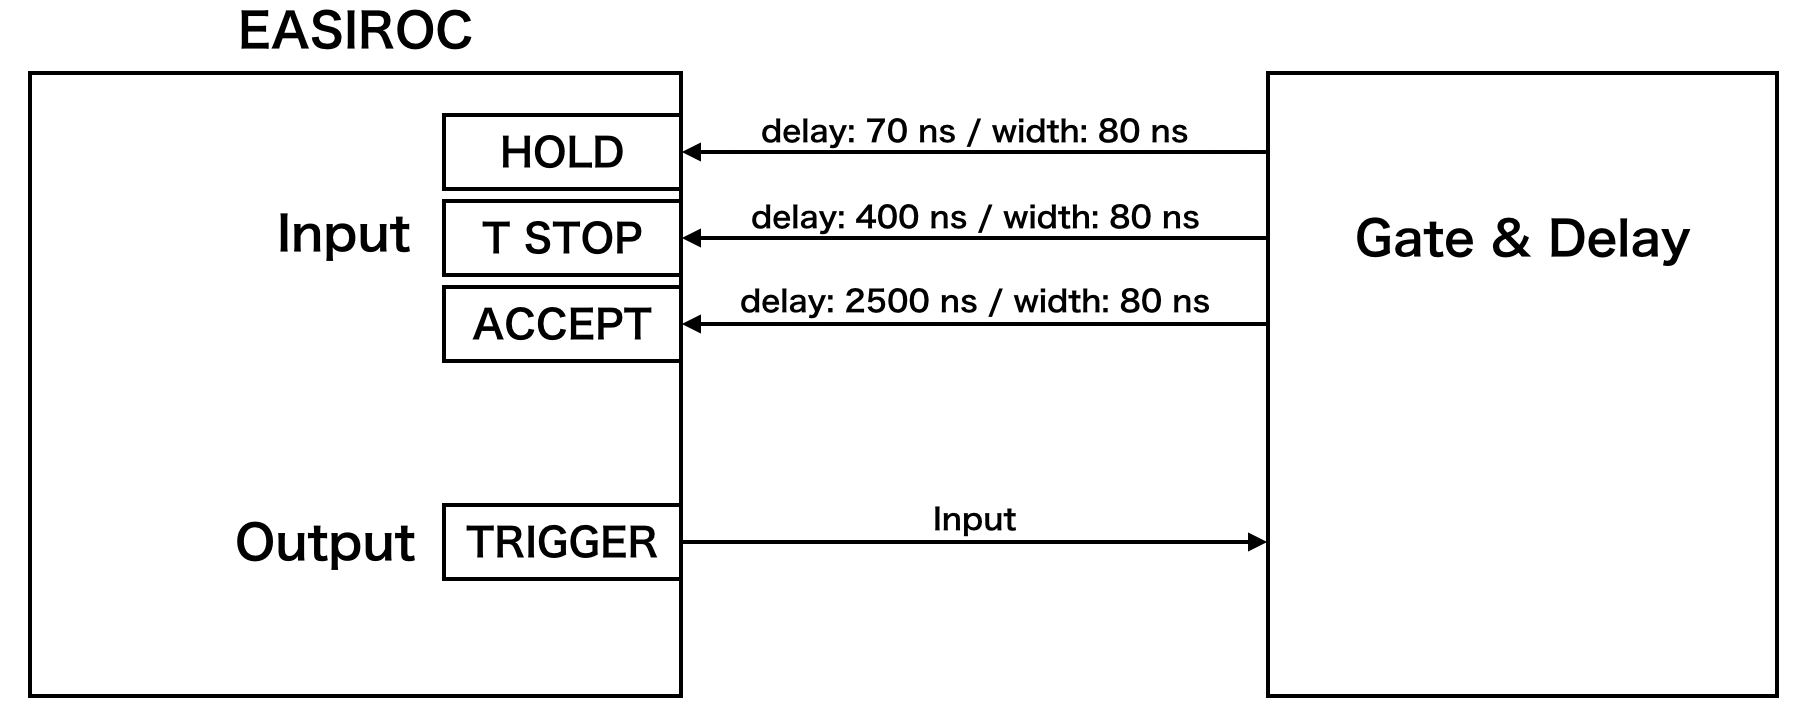
\includegraphics[width = 13.0cm, bb= 0 0 899 358]{1.png}
\end{center}
\caption{内部トリガー信号回路の一例[1]}
\label{fig:}
\end{figure}

\begin{figure}[H]
\begin{center}
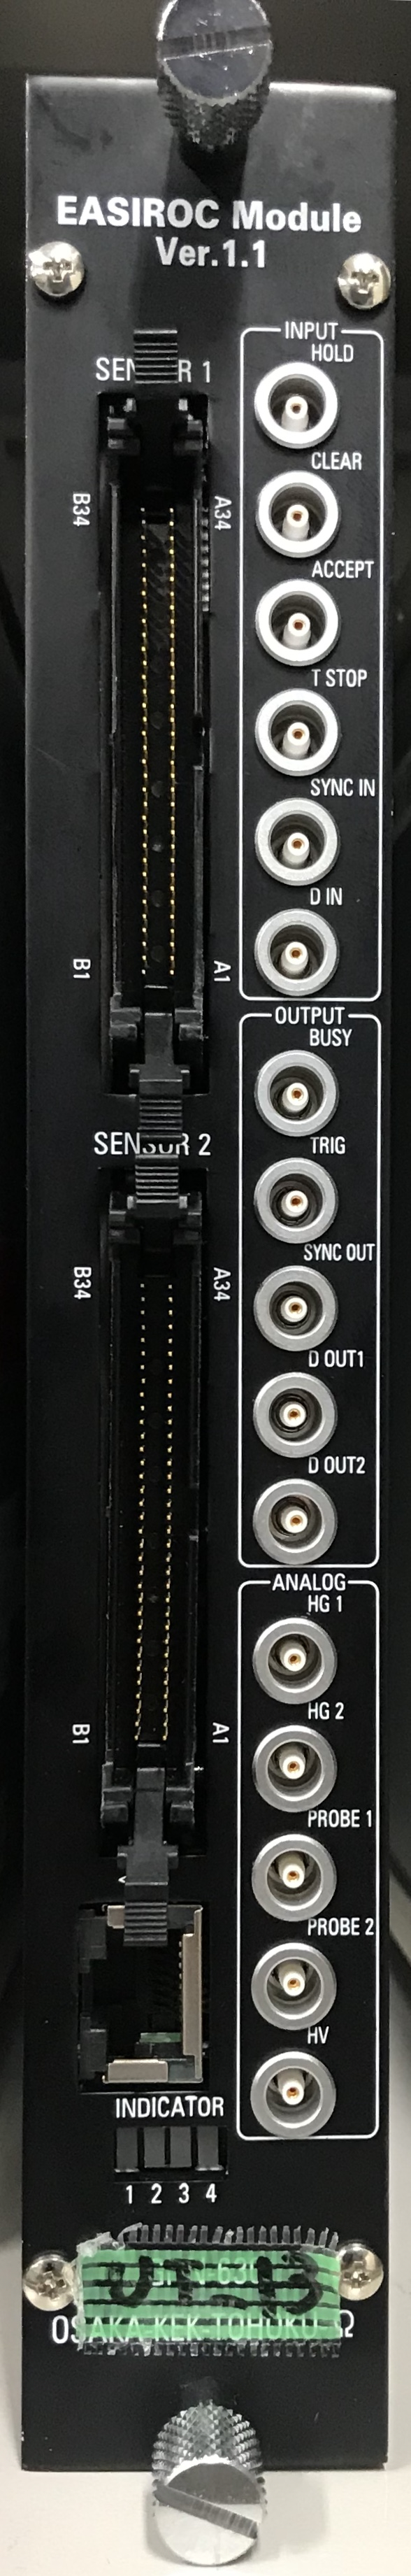
\includegraphics[width = 1.3cm, bb= 0 0 588 3683]{4.jpg}
\end{center}
\caption{EASIROC ボードのフロントパネル}
\label{fig:}
\end{figure}

\newpage
\subsection{対話モード}
内部で Readline が動いており、対話的に EASIROC を操作できる。
\subsubsection{対話モード}
EASIROC対話モードの起動
\begin{shadebox}
\begin{verbatim}
$ ./Controller.rb [IP Address (default: 192.168.10.16)]
\end{verbatim}
\end{shadebox}
 \\
EASIROC対話モードの終了
\begin{shadebox}
\begin{verbatim}
> exit [quit]
\end{verbatim}
\end{shadebox}


\subsubsection{バイアス電圧の設定}

HVの電圧と電流値を表示する
\begin{shadebox}
\begin{verbatim}
> statusHV
\end{verbatim}
\end{shadebox}
 \\
HVを[bias voltage]の値に設定する
\begin{shadebox}
\begin{verbatim}
> setHV [bias voltage]
\end{verbatim}
\end{shadebox}
 \\
HVを[bias voltage]の値まで複数回のstepで上昇。各stepで電流値を確認しリミットに到達したらstopする。
\begin{shadebox}
\begin{verbatim}
> increaseHV [bias voltage]
\end{verbatim}
\end{shadebox}

\subsubsection{データ取得に関わる操作}
Slow controllの値を反映する
\begin{shadebox}
\begin{verbatim}
> slowcontrol
\end{verbatim}
\end{shadebox}
 \\
データ取得を行う
\begin{shadebox}
\begin{verbatim}
> read [Event #] [Filename]
\end{verbatim}
\end{shadebox}
 \\
ADC [TDC/Scaler] をON/OFFにする
\begin{shadebox}
\begin{verbatim}
> adc [on/off]
> tdc [on/off]
> scaler [on/off]
\end{verbatim}
\end{shadebox}
使わないときはOFFにすることでデータ取得が高速になる。

\subsubsection{諸々の情報}
\begin{itemize}
\item 対話時に入力されたコマンドは CommandDispatcher クラスによって処理される
\item 対話モードでhelp と入力してヘルプが見られる
\item 各コマンドは変数 COMMANDS に含まれているものが利用可能で、それぞれのコマンドはメソッドによって処理される
\item シェルのコマンドも一部使えるようになっている(ex. ls, mv, root)
\item それらは変数 DIRECT\_COMMANDS に含まれているものが利用可能
\item Controller ディレクトリ内で hist.cc を make してプログラムを生成していれば、read 終了後に自動でヒストグラムを生成する。出力先は Controller/data ディレクトリ内。
\end{itemize}

\newpage
\subsection{Slow Controll}
Slow Controll は yaml ディレクトリ下の YAML ファイル(拡張子:yml)によって指定される。\\
YAML は構造化されたデータを表現するフォーマットで、XML と似ているが YAML の方が人間にとって理解しやすい形式になっている。よく使いそうなものを以下に紹介する。

\subsubsection{RegisterValue.yml}

\begin{shadebox}
\begin{verbatim}
EASIROC1:  # チップごとに設定
         Capacitor HG PA Fdbck: 100fF    # 増幅率を決定。キャパシタの値は
         Capacitor LG PA Fdbck: 100fF    # RegisterValueAlias.yml に含まれる。
         Time Constant HG Shaper: 100ns  # SlowShaper の時定数
         Time Constant LG Shaper: 50ns
         DAC code: 600  # FastShaper 後段の Discriminator の閾値
 
EASIROC2:
         Capacitor HG PA Fdbck: same
         Capacitor LG PA Fdbck: same
         Time Constant HG Shaper: same
         Time Constant LG Shaper: same
         DAC code: same
 
High Gain Channel 1: 0   # HG1/HG2 で読み出すチャンネルの指定。
High Gain Channel 2: -1  # 読み出すなら0、読み出さないなら-1。
Probe Channel 1: -1      # フロントパネルの Probe からの出力チャンネル選択
Probe Channel 2: -1
Probe 1: Out_fs
Probe 2: Out_fs  # Out_PA_HG, Out_PA_LG, Out_ssh_HG, Out_ssh_LG, Out_fs
SelectableLogic:
         Pattern: Or64        # OneCh_#, Or32u, Or32d, Or64, Or32And,...
         HitNum Threshold: 4  # Threshold for each OR logic. 0~64. Default: 0
         And Channels: -1     # Cannels used in And Logic. 0~63. Default: -1
TimeWindow: 4095ns
UsrClkOut: "OFF"  # フロントパネルの syn out から出力される周期信号 # "ON", 1Hz,...
Trigger:          ## This "Trigger" values are not used for this version.
         Mode: 0  #0-7
         DelayTrigger: -1   #500MHz #default:-1, 0-253 #trig -> hold -> l1 -> l2
         DelayHold: -1      #25MHz
         DelayL1Trig: -1    #6MHz
         Width: raw
\end{verbatim}
\end{shadebox}
Discriminator の DAC 値を大きくするとThreshold は下がる。

\subsubsection{InputDAC.yml}
8-bit Input DACの値がチップごとに32ch分並んでいる。256 - 511 で調整(最上位ビットはenableのため常に1)。\\
DAC 値を上げるとバイアス電圧は小さくなる。
\begin{shadebox}
\begin{verbatim}
---
EASIROC1:
  Input 8-bit DAC:
  - 350
  - 350
  - 350
  - 350
  - 350
  - 350
  - 350
  - 350
\end{verbatim}
\end{shadebox}

\subsubsection{Calibration.yml}

\begin{shadebox}
\begin{verbatim}
HVControl:   # 指定した HV を DAC 値に変換する係数
        - 413.9 #423.06 #483.183
        - 747.8 #767.17 #780.0
MonitorADC:  # Monitor ADC で読み取った値を電圧、電流、温度に変換する係数
        HV: 0.00208 #0.3235 #0.00208
        HVOffset: 0.0355 #4.1694
        Current: 0.0364 #0.034
        InputDac: 0.00006866 #4.5/2^16 #0.0000685
        Temperature: 4500.0
\end{verbatim}
\end{shadebox}
